\scanpage{62}
On trouve
\[
\operatorname{Aut}^0(C,a)\simeq\prod_{x\in C_0\setminus\{a\}}\deleted{\unsure{G_x}}\pi_x
\]

\figure{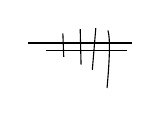
\begin{tikzpicture}[x=0.22cm,y=0.22cm]
\draw (-3,0)--(3,0) (-2,-.45)--(2.7,-.45);
\draw (-1,.55)--(-.95,-.8) (0,.8)--(.05,-1.25) (.9,.85)--(.7,-1.56) (1.6,.72) .. controls (1.8,.1) and (1.6,-2) .. (1.55,-2.6);
\end{tikzpicture}}

\deleted{Soit $K$ \unsure{un|le|des} graphe\unsure{,|.}}

Soit $I$ un ensemble muni d'une structure polygonale d'ordre $n\geq2$ \deleted{\unsure{i.e.} \unsure{$A_o$}} [pour $n=2$, il faut se donner l'un des \unsure{orbites|orientés} \inserted{de cardinal 2} $\deleted{\unsure{\Delta}}I^*$, \deleted{de cardinal 2, et} ou ce qui revient au $=$, $\Omega(\Pi)\simeq I\mathbin{\wedge}I^*\ \ldots$ ], $\mathbb D\ (\simeq\mathbb D_n)$ le groupe des autom. de $I$.

Soit $K=K(I)$ le graphe donné par
\[
\begin{aligned}
&\text{\uline{sommets} :}& \deleted{\unsure{O}}\Omega(\Pi)&=C_0=\{o,o'\}\\
&\text{\uline{arêtes}}& I&:\quad\text{(indexation $(\unsure{\ell|b}_i)_{i\in I}$)}
\end{aligned}
\]
\deleted{\unsure{Relation} d'incidence}

Incidence : \quad $C_0\times I$ (\unsure{tte|tt} arête incidente à \deleted{\unsure{tt o}}\inserted{tt sommet})

\inserted{$G$ opère sur $K(I)$, et on a aussi \deleted{\unsure{autre}} \inserted{l'involution} $\tau$ qui est l'identité sur $I$, et échange $o,o'$, commutant à $G$.}

\diagram{\begin{tikzcd}[ampersand replacement=\&,row sep=huge]
o\arrow[d,bend left=62,dash,"\ell_1"]\arrow[d,bend right=34,dash,double,swap,"\ell_0"]\arrow[d,bend right=61,dash,swap,"\ell_2"]\\
o'
\end{tikzcd}}

Soit $C(I)$ le groupoïde fondamental \unsure{du|de} $K(I)$. \deleted{le \unsure{gpe}} $G$ y opère par automorphismes, en opérant transitivement sur $C_0=\{o,o'\}$.

On va regarder le \deleted{commutant}\inserted{normalisateur de $G$} dans
% archive sheet number: 61
